\documentclass[fontsize=12pt,paper=a4,twoside]{scrartcl}

\newcommand{\grad}{\ensuremath{^{\circ}} }
\renewcommand{\strut}{\vrule width 0pt height5mm depth2mm}

\usepackage[utf8]{inputenc}
\usepackage[final]{pdfpages}
% obere Seitenränder gestalten können
\usepackage{fancyhdr}
\usepackage{moreverb}
% Graphiken als jpg, png etc. einbinden können
\usepackage{graphicx}
%\usepackage{stmaryrd}
% Floats Objekte mit [H] festsetzen
\usepackage{float}
% setzt URLs schön mit \url{http://bla.laber.com/~mypage}
\usepackage{url}
% Externe PDF's einbinden können
\usepackage{pdflscape}
% Verweise innerhalb des Dokuments schick mit " ... auf Seite ... "
% automatisch versehen. Dazu \vref{labelname} benutzen
\usepackage[ngerman]{varioref}
\usepackage[ngerman]{babel}
\usepackage{ngerman}
% Bibliographie
\usepackage{bibgerm}
% Tabellen
\usepackage{tabularx}
\usepackage{supertabular}
\usepackage[colorlinks=true, pdfstartview=FitV, linkcolor=blue,
            citecolor=blue, urlcolor=blue, hyperfigures=true,
            pdftex=true]{hyperref}
\usepackage{bookmark}

\newboolean{langversion} %Deklaration
\setboolean{langversion}{true} %Zuweisung ist 'false' für Blockkurs
\newcommand{\highlight}[1]{\textcolor{blue}{\textbf{#1}}}
\newcommand{\nurlangversion}[0]{%
\ifthenelse{\boolean{langversion}}{\highlight{}}{\highlight{Entfällt in SWP-1}}}

\newcommand{\swp}[0]{\ifthenelse{\boolean{langversion}}%
{Software--Projekt 2}{Software--Projekt 1}}
\newcommand{\jahr}[0]{2014 (RE SWP)}
\newcommand{\semester}[0]{\ifthenelse{\boolean{langversion}}{SoSe}{SoSe} \jahr}

% Damit Latex nicht zu lange Zeilen produziert:
\sloppy
%Uneinheitlicher unterer Seitenrand:
%\raggedbottom

% Kein Erstzeileneinzug beim Absatzanfang
% Sieht aber nur gut aus, wenn man zwischen Absätzen viel Platz einbaut
\setlength{\parindent}{0ex}

% Abstand zwischen zwei Absätzen
\setlength{\parskip}{1ex}

% Seitenränder für Korrekturen verändern
\addtolength{\evensidemargin}{-1cm}
\addtolength{\oddsidemargin}{1cm}

\bibliographystyle{gerapali}

% Lustige Header auf den Seiten
  \pagestyle{fancy}
  \setlength{\headheight}{70.55003pt}
  \fancyhead{}
  \fancyhead[LO,RE]{\swp\\ \semester{}
  \\Anforderungsspezifikation}
  \fancyhead[LE,RO]{Seite \thepage\\\slshape \leftmark\\\slshape \rightmark}

%
% Und jetzt geht das Dokument los....
%

\begin{document}

% Lustige Header nur auf dieser Seite
  \thispagestyle{fancy}
  \fancyhead[LO,RE]{ }
  \fancyhead[LE,RO]{Universität Bremen\\FB 3 -- Informatik\\
  Dr. Karsten Hölscher \\Tutor: Karsten Hölscher}
  \fancyfoot[C]{}

% Start Titelseite
  \vspace{3cm}

  \begin{minipage}[H]{\textwidth}
  \begin{center}
  \bf
  \Large
  \swp{} \jahr\\
  \smallskip
  \small
  VAK 03-BA-901.02\\
  \vspace{3cm}
  \end{center}
  \end{minipage}
  \begin{minipage}[H]{\textwidth}
  \begin{center}
  \vspace{1cm}
  \bf
  {\Large Anforderungsspezifikation}\\
  \vspace{3ex}
  Schibboleth\\
  
\includegraphics[width=0.6\textwidth]{Bilder/Logo.png}
  \vfill
  \end{center}
  \end{minipage}
  \vfill
  \begin{minipage}[H]{\textwidth}
  \begin{center}
  \sf
  \begin{tabular}{lrr}
  Patrick Hollatz & phollatz@tzi.de & 2596537 \\
  Tobias Dellert & tode@tzi.de & 2936941 \\
  Tim Ellhoff & tellhoff@tzi.de & 2520913\\
  Daniel Pupat & dpupat@tzi.de & 2703053 \\
  Olga Miloevich & halfelv@tzi.de  & 2586817\\  
  Tim Wiechers & tim3@tzi.de & 2925222 \\
  \end{tabular}
  \\ ~
  \vspace{2cm}
  \\
  \it Abgabe: 01.06.2014 --- Version 1.7\\ ~
  \end{center}
  \end{minipage}

% Ende Titelseite

% Start Leerseite

\newpage

  \thispagestyle{fancy}
  \fancyhead{}
  \fancyhead[LO,RE]{\swp{}\\ \semester{}
  \\Anforderungsspezifikation}
  \fancyhead[LE,RO]{Seite \thepage\\\slshape \leftmark\\~}
  \fancyfoot{}
  \renewcommand{\headrulewidth}{0.4pt}
  \tableofcontents

\newpage

  \fancyhead[LE,RO]{Seite \thepage\\\slshape \leftmark\\\slshape \rightmark}


%%%%%%%%%%%%%%%%%%%%%%%%%%%%%%%%%%%%%%%%%%%%%%%%%%%%%%%%%%%%%%%%%%%%%%%%
\section*{Version und Änderungsgeschichte}


\begin{tabular}{ccl}
Version & Datum & Änderungen \\
\hline
1.0 & 21.05.2014 & Analyse ähnlicher Systeme. \\
1.1 & 22.05.2014 & Anwendungsfälle  \\
1.2 & 27.05.2014 & Ist-Analyse \\
1.3 & 28.05.2014 & Produktperspektiven \\
1.4 & 29.05.2014 & Einschränkungen \\
1.5 & 30.05.2014 & Annahmen und Abhängigkeiten \\
1.6 & 30.05.2014 & Ausblick \\
1.7 & 30.05.2014 & Charakteristika der Benutzer \\

\end{tabular}


%%%%%%%%%%%%%%%%%%%%%%%%%%%%%%%%%%%%%%%%%%%%%%%%%%%%%%%%%%%%%%%%%%%%%%%%

\paragraph{Wichtiger Hinweis:} Diese Anforderungsspezifikation wurde zu einem Teil aus verschiedenen Dokumententeilen der Anforderungsspezifikation unserer Gruppenmitglieder aus dem Wintersemester 2013/14 erstellt (Gruppe \textit{IT\_R3V0LUTION}). Einige Teile wurden komplett übernommen, andere überarbeitet bzw. angepasst. \\
Diese Vereinbarung haben wir in der Kick-Off-Veranstaltung für RE SWP 2014 mit dem Veranstalter Dr. Karsten Hölscher getroffen. \\
\section{Einleitung (Patrick)}
\nurlangversion

{\em Dieses Dokument dient als Vorlage für Eure
  Anforderungsspezifikation. Die Gliederung dieses
  Dokuments ist an die Struktur des IEEE-Standards 830.1998 angelehnt,
  weicht jedoch an einigen Stellen davon ab. Die Abweichungen sind
  im weiteren Verlauf dieses Dokuments dokumentiert. Weitere detaillierte
  Hinweise finden sich im IEEE-Standard 830.1998, der in Stud.IP      
  beziehungsweise über die Uni-Bibliothek in digitaler Form verfügbar ist
  \footnote{Bei \url{http://ieeexplore.ieee.org} im Suchfeld 'IEEE std    
   830-1998' eingeben. Funktioniert nur innerhalb des Uni-Netzes.}.}

\subsection{Zweck}
\nurlangversion

  {\em Was ist der Zweck dieser Anforderungsspezifikation? Wer sind
  die LeserInnen?}

\subsection{Rahmen}
\nurlangversion

  {\em Dieser Abschnitt soll einen groben Überblick über die zu
  erstellende Software geben: Welche Produkte sind zu erstellen (mit
  Namen)? Was tut die Software? Auch: Was tut sie nicht? Wozu soll die
  Software verwendet werden?  (Ziele etc.)}

\subsection{Definitionen, Akronyme und Abkürzungen}
\nurlangversion

  {\em Hier geht es vor allem um Begriffe aus der Anwendungsdomäne,
  d.h.\ aus der Welt des Kunden. Aber auch Begriffe, die dem Kunden
  evtl.\ fremd oder unklar sind, sollten erläutert werden.}


\subsection{Referenzen}
  {\em Neben sonstigen Quellen, die Ihr verwendet habt, können dies
  z.B.\ das Skript, dieses Beispieldokument, der zugrunde
  liegende IEEE-Standard und anderes sein}
  

\subsection{Übersicht über das Dokument}
\nurlangversion

  {\em Was enthält die Anforderungsspezifikation? Wie ist das Dokument
  organisiert?}


\section{Allgemeine Beschreibung}
\label{ch:AllgemeineBeschreibung}

\subsection{Ergebnisse der Ist-Analyse (Tim E.)}
  
Das Rektorat der Universität Bremen möchte aus Eigeninteresse und auch als Werbung Menschen und insbesondere Studieninteressierte, aber auch Studierende und Mitarbeitern die Uni in drei Bereichen näher bringen: Campusleben, Studium und Forschung. Dabei soll insbesondere der Bezug zum Studienort hergestellt werden.\\
Um dies zu erreichen, möchte die Universität gerne eine Quiz-App veröffentlichen und bereitstellen, die von den oben stehenden Interessengruppen gespielt werden kann und Fragen aus den drei Kernbereichen zur Verfügung stellt.\\
Bisher gibt es zwar eine Campus App der Universität, die aber andere Ziele verfolgt und in erster Linie nur für Studierende gedacht ist. Eine spezielle Quiz-App, zugeschnitten auf die Belange der Uni, gibt es allerdings noch nicht. \\
Unser Ziel ist es, genau eine solche App zu entwickeln, die benutzerfreundlich, leicht zu bedienen ist und durch ihr ansprechendes GUI-Design auch noch Spaß machen soll. Darüber hinaus wird es eine Administrationswebseite geben, auf der grundlegende Einstellungen konfiguriert werden können und auch eine redaktionelle Bearbeitung der Fragen und Antworten stattfinden kann.\\
Dabei werden die Fragen aus den drei Kategorien von der Pressestelle der Universität zur Verfügung gestellt. \\
Um die genauen Anforderungen und Kundenwünsche an das System über die vom Veranstalter des Software-Projekts 2 erhobenen Mindestanforderungen hinaus zu erfassen, haben wie ein Kundengespräch durchgeführt.

\subsubsection{Erstes Kundengespräch vom 08.05.2014}

Am Donnerstag, den 08.05.2014, um 10:00 Uhr begann unser erstes Kundengespräch mit der Vertreterin des Kunden, Frau Sprindt von der Pressestelle der Universität. In den Tagen zuvor hat die Gruppe Ideen zu einem Fragenkatalog gesammelt, der dann am Vortag der Besprechung fertiggestellt wurde. Er beinhaltete eine Auflistung aller Mindestanforderungen, zu denen Unklarheiten bezüglich des Realisierungsvorgangs notiert wurden. 

Das offizielle Gespräch begann pünktlich um 10:00 Uhr. Leider gab es keine wirkliche Ordnung bei den gestellten Fragen, was es etwas schwer machte, die einzelnen Vorgänge strukturiert zu durchdenken.\\
Grundsätzlich soll sich die App an die bekannte Quiz-App \textit{Quizduell} anlehnen bzw. als eine Art Vorbild genommen werden. Genaueres dazu findet man im Abschnitt \ref{quizduell}, wo die Analyse eines bestehenden Systems vorgenommen wird.

\subsubsection{Auswertung des Kundengesprächs}

Es haben sich im Kundengespräch jedoch keine großen Überraschungen oder unerwartete Kundenwünsche oder -änderungen ergeben, die über die Mindestanforderungen besonders hinaus gehen. Einige Besonderheiten sollen aber im Folgenden näher beschrieben werden.\\

Man soll die App auch ohne Registrierung spielen können, allerdings nur lokal auf einem Gerät. Man hat dann nicht die Möglichkeit, später woanders weiterzuspielen. Das soll nur funktionieren, wenn man sich als Nutzer mit Benutzernamen und Passwort registriert hat, wobei es eine Benutzernamenkontrolle geben soll, die unpassende Namen verbietet. Auch soll der Admin jederzeit unpassende Benutzer über den Admin-Zugang löschen oder ändern können.\\
Es soll bis zu 10 parallel laufende Spiele geben können, wobei dieser Wert vom Admin editiert werden kann. Ebenso sollen die Spiele zeitversetzt gespielt werden können. Drei Fragen pro Runde sind vorgesehen, wobei ein Zeitlimit von 10-30 Sekunden eingeplant ist (die tatsächliche Antwortzeit sollte man in einem Praxistest genauer ermitteln).\\
Es wurde besonderen Wert darauf gelegt, dass in der GUI-Gestaltung das Corporate Design der Universität Bremen mit einbezogen wird, sodass z.B. durch Einfügen des Uni-Logos ein Wiedererkennungswert und ein direkter Bezug zur Uni bei den Nutzern hergestellt wird. Auch ein Verweis auf die Universität-Webseite sowie ggf. eine Social-Media-Anbindung sind erwünscht, wenn auch eher optionaler Art.\\
Die Spieler sollen geduzt werden und möglichst gender-neutral, sofern sinnvoll und möglich, angesprochen werden.\\
Auch die Einbindung von wohlklingenden und passenden Sounds soll den Spaß am Spiel wecken.\\
Des Weiteren sollen im Spiel selbst zu jeder Frage vier Antwortmöglichkeiten gegeben werden und Joker in Form eines 50:50-Jokers oder einer Zeitverlängerung eingebaut werden, die man sich jedoch erst erspielen muss und nicht von Beginn an zur Verfügung stehen.\\
Der Schwierigkeitsgrad steigt nicht mit jeder Frage, sondern die Fragen werden nach Kategorie, die die Spieler zu Beginn bestimmen können, zufällig ausgewählt. \\
Wenn ein Spieler aufgibt bzw. das laufende Spiel abbricht, soll er in Form eines Punktabzugs bestraft werden. \\
Es soll allerdings keine Freundes- oder Rivalenlisten geben. 



\subsubsection{Analyse eines ähnlichem Systems (Daniel Pupat)}\label{quizduell}

Als System haben wir uns die App \textit{Quizduell} ausgesucht. Die App ist im App-Store kostenlos zu erhalten. Wir benutzen hierzu nicht die Premium-Version, da die kostenlose unserem System am nächsten kommt. Wir haben nicht die Rechte eines Administrators, weshalb sich die Analyse nur auf die App bezieht. Die App kann nur verwendet werden, wenn man eine bestehende Internetverbindung hat.\\

\begin{figure}[H]
\centering

\includegraphics[scale=0.5]{Bilder/lade.png}
\caption{Ladebildschirm}
\end{figure}

Dies ist der Ladebildschirm, sobald die App gestartet wird.

\begin{figure}[H]
\centering
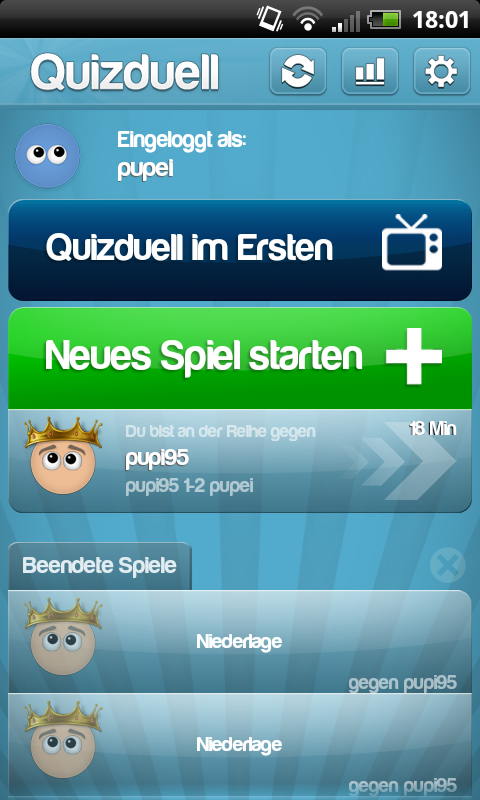
\includegraphics[scale=0.5]{Bilder/start.png}
\caption{Startbildschirm}
\end{figure}

Hier ist der Startbildschirm, nachdem man eingeloggt ist. Oben hat man die Funktionen Aktualisieren, Statistiken und Einstellungen. Beim Aktualisieren wird die Seite aktualisiert. \\

\begin{figure}[H]
\centering
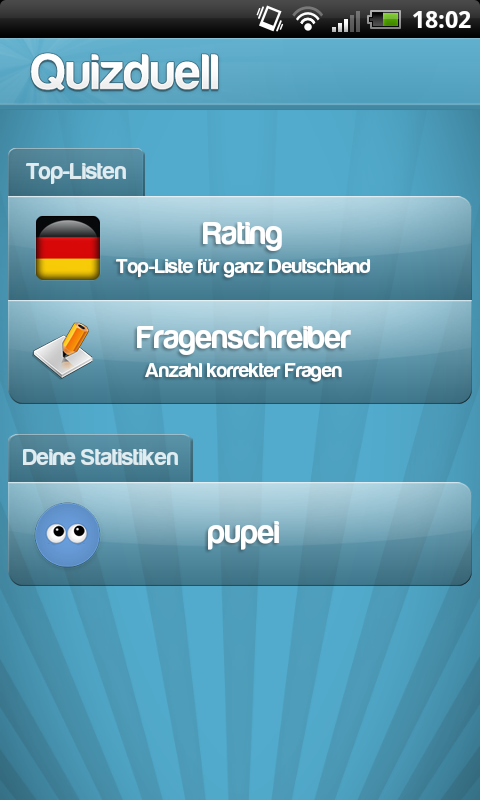
\includegraphics[scale=0.5]{Bilder/stat.png}
\caption{Statistiken}
\end{figure}

Hier kann man die Rating Liste aller Nutzer in Deutschland im Bezug auf der Punktzahl und der Anzahl der geschrieben und angenommenen Fragen sehen. Für die eigene Statistik wird eine Premium-Version benötigt.\\

\begin{figure}[H]
\centering
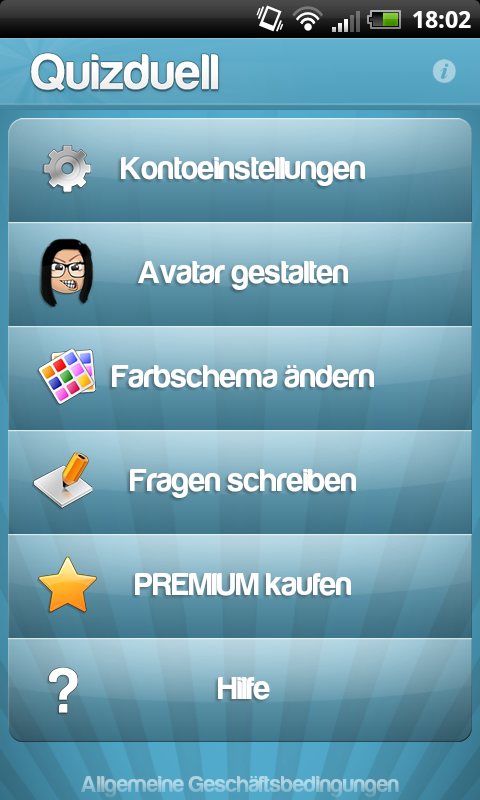
\includegraphics[scale=0.5]{Bilder/optionen.png}
\caption{Einstellungen}
\end{figure}

Unter Einstellungen kann man seine Kontoeinstellungen bearbeiten, wo man den Benutzernamen und Passwort ändern kann. Für Avatar gestalten und Farbschema ändern beötigt man die Premium-Version, welche man unter PREMIUM kaufen erwerben kann. Bei Fragen schreiben, kann man eigene Fragen schreiben, die evtl. dann übernommen werden. Bei Hilfe werden bestimmte Fragen im Hinblick auf die Benutzung beantwortet.\\

\begin{figure}[H]
\centering
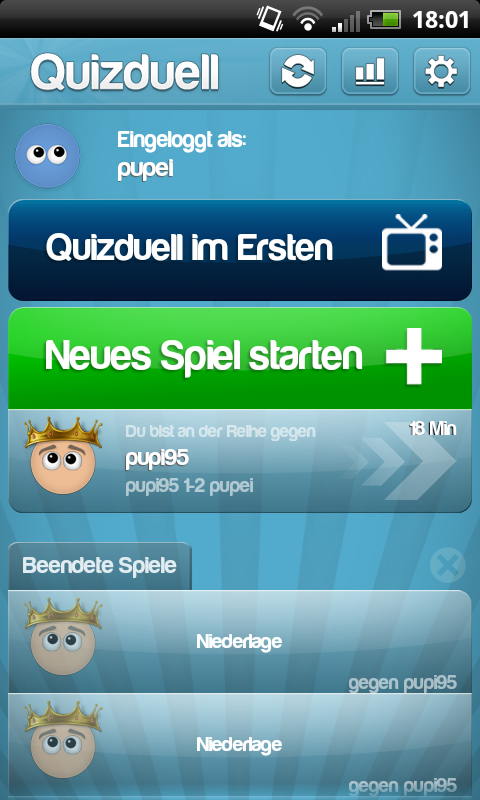
\includegraphics[scale=0.5]{Bilder/start.png}
\caption{Startbildschirm}
\end{figure}

Weitere Funktionen beim Startbildschirm sind Neues Spiel starten oder ein bereits angefangenes Spiel weiterspielen.\\

\begin{figure}[H]
\centering
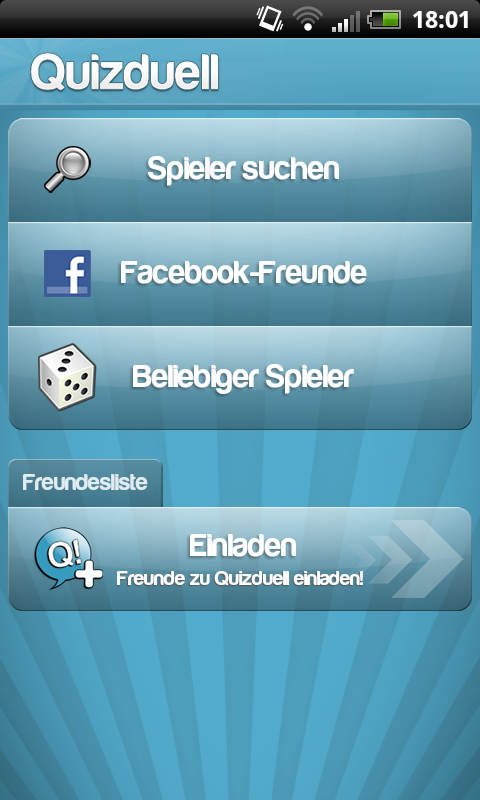
\includegraphics[scale=0.5]{Bilder/neuesspiel.png}
\caption{Bildschirm wenn man ein neues Spiel starten möchte}
\end{figure}

Wenn man ein neues Spiel starten möchte, kann man einen neuen Spieler suchen, unter Facebook Freunden suchen, falls man unter Facebook eingeloggt ist, oder gegen einen beliebigen Spieler spielen, der ebenfalls einen gesucht hat. 


\begin{figure}[H]
\centering
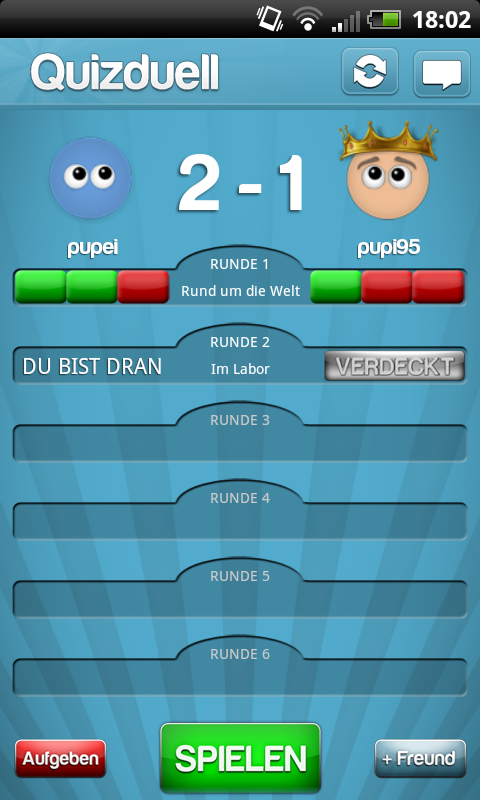
\includegraphics[scale=0.5]{Bilder/spiel.png}
\caption{Bildschirm beim neuen oder laufenden Spiel}
\end{figure}

Hier wird der bisherige Spielstand angezeigt. Insgesamt gibt es 6 Fragen, welche jeder beantworten muss. Die Spieler erhalten jeweils die gleichen Fragen. Es werden immer 2 Fragen abwechselnd gestellt, wobei der Spieler einmal eine Kategorie auswählen darf und einmal die Fragen der Kategorie des Gegners beantworten muss. Die Spieler haben 48 Stunden Zeit, die Fragen zu beantworten, bis das Spiel automatisch mit einer Niederlage des Spielers, der nicht geantwortet hat, endet. 

\begin{figure}[H]
\centering
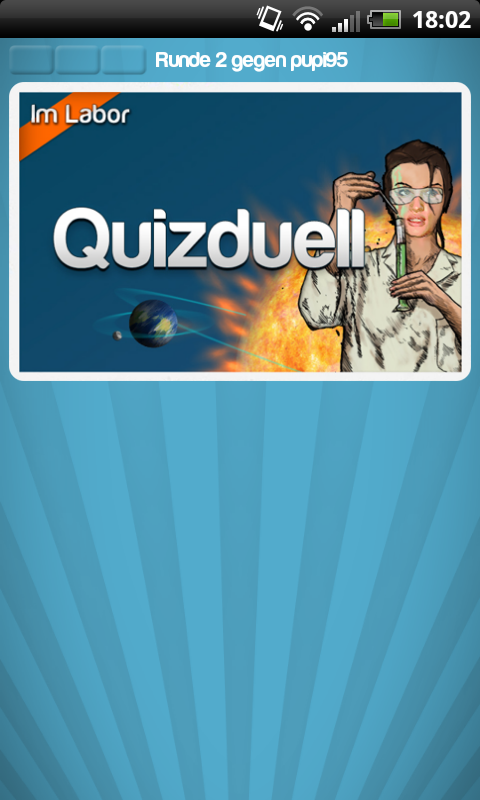
\includegraphics[scale=0.5]{Bilder/spielstart.png}
\caption{Beim Starten der Fragen}
\end{figure}

Beim Starten einer Frage erscheint erst nur eine Karte mit der Kategorie, bei einer Berührung wird die Karte umgedreht.\\

\begin{figure}[H]
\centering
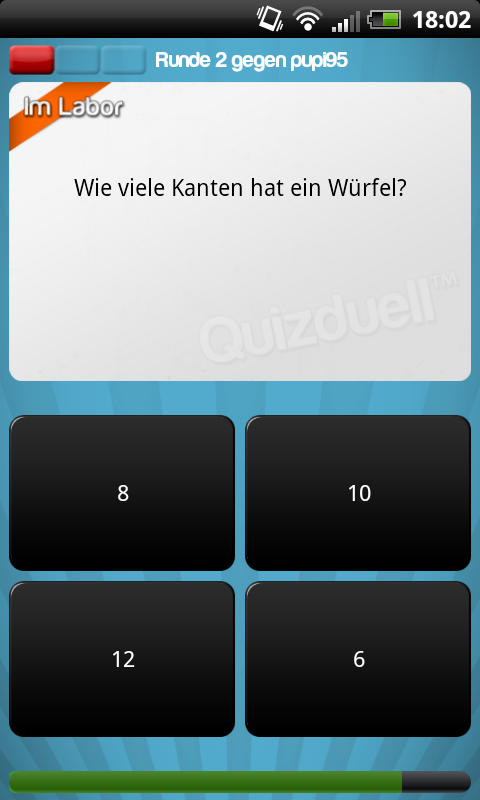
\includegraphics[scale=0.5]{Bilder/frage.png}
\caption{Anzeigen der Frage}
\end{figure}

Nun wird die Frage angezeigt, man hat 20 Sekunden Zeit, um die Frage zu beantworten, sonst wird diese als falsch gewertet.\\

\begin{figure}[H]
\centering
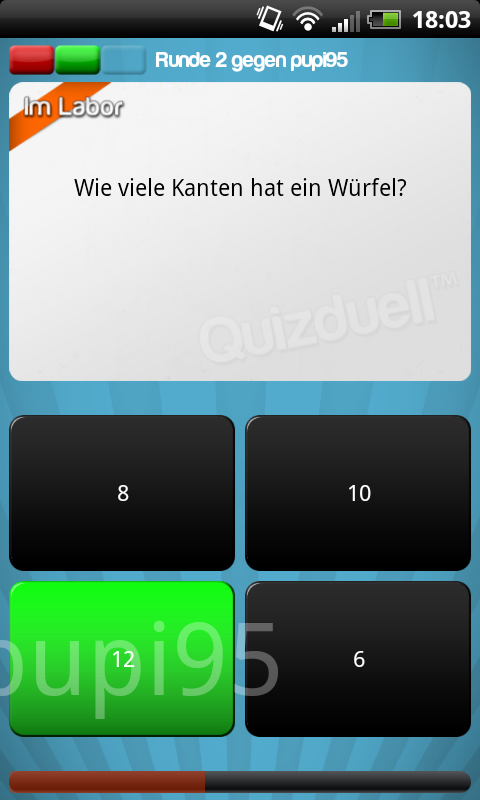
\includegraphics[scale=0.5]{Bilder/antwort.png}
\caption{Reaktion bei richtiger Antwort}
\end{figure}

Bei einer richtigen Antwort wird diese mit Grün unterlegt und zeitgleich wird der Name des Gegners auf seiner Antwort angezeigt, wenn er diese bereits beantwortet hat. Bei einer falschen wird die Antwort mit rot unterlegt.\\

\textbf{Fazit:}\\
Die \textit{Quizduell} App ist ein gutes System, mit welcher man unseres später vergleichen kann. Es hat viele Funktion, wie gezeigt, welche unser System ebenfalls haben muss. Es gibt allerdings auch Unterschiede. In unserer App wird es nur 3 Fragen pro Runde geben und es werden keine eigenen Fragen geschrieben, außerdem wird es keine Premium-Version geben. Zudem werden wir auch Offline-Funktion einbauen, in welcher der Spieler alleine spielen kann.\\ 

\subsection{Produktperspektive (Tim W. und Tim E.)}
  
\subsubsection{Systemschnittstellen}
  
Als Grundlage dient ein neu aufzusetzendes oder bestehendes System, auf dem die Software installiert werden kann. Als externe Schnittstelle muss dieses mit dem Internet verbunden sein. Der Server der Quizapp kann an einem PC über HTTP mit einem HTML5-unterstützenden Browser angesprochen werden. Mobiler Zugriff erfolgt auf Android-Geräten zudem mit einer eigenen App.

\subsubsection{Benutzerschnittstelle}

Die GUI der Website weist je nachdem, ob sich ein normaler Nutzer oder ein Admin anmeldet, unterschiedliche Funktionalitäten auf. 

\subsubsection{Hardwareschnittstellen}

Die HTML-Website ist plattform-unabhängig nutzbar. Smartphones mit kompatibler Android-Version (welche?) können die Quizapp nutzen.


\subsubsection{Softwareschnittstellen}

  \begin{tabular}{|l|l|l|l|}\hline
    \textbf{Name} & \textbf{Version} & \textbf{Hersteller} & \textbf{Quelle} \\\hline
    Java Runtime & 6 Update 37 & Oracle & \url{http://java.com} \\\hline
    JUnit & & & \\\hline
    libGDX &  &  & \\\hline
    Android & & & \\\hline
  \end{tabular}

\subsubsection{Kommunikationsschnittstellen}
  
Das System muss mit einer öffentlichen IP-Adresse und Domain von außen ansprechbar sein. Die Bandbreite sollte groß genug sein, um mehreren Nutzern parallel den Zugang zur Software zu gewähren, wobei jeder Nutzer einzeln nur eine sehr geringe Bandbreite benötigt.

\subsubsection{Speicherbeschränkung}


Die App wird voraussichtlich bis zu 30 MB Speicherplatz beziehen. (Arbeitsspeicher?)


\subsubsection{Operationen (Betriebsmodi)}

Wir unterscheiden zwischen dem normalen Betriebsmodus und einem Wartungsmodus, in dem z.B. Backups aufgespielt werden können. Während des Wartungsmodus ist kein öffentlicher Zugriff vorgesehen. Im normalen Betriebsmodus wird unterschieden zwischen Admins, registrierten Benutzern und Gästen. Jeder hat das Recht zu spielen, wobei registrierte Nutzer Vorteile wie Statistiken etc. genießen. Der Admin kann das System über die Website verwalten, z.B. Nutzernamen ändern. In der App ist kein Admin-Modus vorhanden.

\subsubsection{Möglichkeiten der lokalen Anpassung}
  
Es handelt sich bei dem System um ein lauffähiges Gesamtpaket. Es muss keine Datenbank o.Ä. eingerichtet werden. Lediglich eine IP-Adresse muss eingerichtet werden. Somit ist keine lokale Anpassung nötig.

\subsection{Anwendungsfälle (Daniel)}
\begin{itemize}
	\item \textbf{1. App starten}\\
	Die App wird gestartet. 
	\item \textbf{2. Offline-Modus starten}\\
	Die App wird im Offline-Modus gestartet. Keine Anmeldung und Internet Verbindung notwendig.
	\item \textbf{3. Benutzer registrieren}\\
	Benutzer registriert sich mit Benutzernamen und Passwort
	\item \textbf{4. Benutzer anmelden}\\
	Der Benutzer meldet sich mit Benutzernamen und Passwort an. Die Daten werden gespeichert, sodass kein nochmaliges anmelden nötig ist.
	\item \textbf{5. Benutzer abmelden}\\
	Benutzer wird abgemeldet und muss sich beim nächsten Start wieder anmelden.
	\item \textbf{6. Online Modus starten}\\
	Der Online Modus wird gestartet. Einmaliges anmelden und Internet Verbindung erforderlich.
	\item \textbf{7. Neues Spiel starten}\\
	Eine Liste aller Spieler die online sind wird angezeigt.
	\item \textbf{8. Gegner herausfordern}\\
	Aus der Liste kann ein Spieler angeklickt und herausgefordert werden.
	\item \textbf{9. Herausforderung annehmen}\\
	Bei einer Herausforderung kann der Gegner annehmen oder ablehnen.
	\item \textbf{10. Spielrunde starten}\\
	Eine neue Spielrunde wird gestartet, die erste Frage erscheint.
	\item \textbf{11. Frage beantworten}\\
	Der Spieler hat 20 Sekunden Zeit zu antworten.
	\item \textbf{12. Einstellungen ändern}\\
	Unter Einstellungen kann der Benutzername und das Passwort geändert werden
	\item \textbf{13. Punktzahl anzeigen}\\
	Rangliste mit den Punktzahlen aller Mitspieler wird angezeigt
	\item \textbf{14. Website wird aufgerufen}\\
	Website wird angezeigt.
	\item \textbf{15. Admin anmelden}\\
	Benutzer meldet sich als Admin an. Die Website ist nur für Administratoren verwendbar.
	\item \textbf{16. Admin abmelden}\\
	Benutzer meldet sich als Admin ab.
	\item \textbf{17. Frage hinzufügen}\\
	Eine neue Frage wird hinzugefügt
	\item \textbf{18. Frage bearbeiten}\\
	Eine vorhandene Frage wird bearbeitet
	\item \textbf{19. Frage löschen}\\
	Eine vorhandene Frage wird gelöscht
	\item \textbf{20. User löschen}\\
	Bestimmter User wird gelöscht
\end{itemize}

\subsection{Charakteristika der Benutzer (Tim W.)}
	\begin{tabular}{|r|l|}\hline
       Name: & Armin Admin\\\hline
       Benutzertyp: & Administrator\\\hline
       Tätigkeit	& Redakteur\\\hline
       Wohnort & Uniallee, Bremen\\\hline
       Alter	 & 42\\\hline
       Motivation & System aufrecht erhalten\\\hline
       Aufgaben & Verwaltung und Systemwartung\\\hline
    \end{tabular}\\
        
    	\begin{tabular}{|r|l|}\hline
       Name: & Paul Neuling\\\hline
       Benutzertyp: & Gelegenheitsspieler \\\hline
       Tätigkeit	& Student\\\hline
       Wohnort & Uniallee, Bremen\\\hline
       Alter	 & 19\\\hline
       Motivation & Etwas über die Uni lernen und Spaß haben\\\hline
    \end{tabular}\\
    
    	\begin{tabular}{|r|l|}\hline
       Name: & Klaus Zocker\\\hline
       Benutzertyp: & Häufiger Spieler \\\hline
       Tätigkeit	& Student\\\hline
       Wohnort & Uniallee, Bremen\\\hline
       Alter	 & 23\\\hline
       Motivation & Will die Rangliste anführen\\\hline
    \end{tabular}\\
    
    \begin{tabular}{|r|l|}\hline
       Name: & Sabine Ohnenetz\\\hline
       Benutzertyp: & Gelegenheitsspielerin \\\hline
       Tätigkeit	& Student\\\hline
       Wohnort & Uniallee, Bremen\\\hline
       Alter	 & 19\\\hline
       Motivation & Offline etwas spielen \\\hline
    \end{tabular}\\
  
  \subsection{Einschränkungen (Tim E.)}

Im Folgenden listen wir die Mindestanforderungen des Produkts auf, die nur mithilfe eines Logins bei StudIP einzusehen sind\footnote{\url{https://elearning.uni-bremen.de/scm.php?cid=2b323f34b16a84e8dce31dcdfc0be6ad\&show\_scm=4c88951a202b2543c96de2c8a476d471}}.

\textbf{Server:}
\begin{itemize}
\item SpielerInnen können sich beim Server registrieren
\item verwaltet eine Liste aller SpielerInnen
\item verwaltet die Fragekategorien, die Fragen und die Antworten sowie Belohnungen
\item SpielerInnen können sich beim Server als gerade spielbereit setzen und wieder entfernen
\item auf Anfrage wird aus der Liste der gerade spielbereiten SpielerInnen zufällig eine konkrete GegnerIn ermittelt
\item verwaltet laufende Spiele und archiviert diese
\begin{itemize}
\item TeilnehmerInnen
\item aktueller Punktestand
\item gestellte Fragen
\item gegebene Antworten
\end{itemize}
\end{itemize}
\begin{itemize}
\item verwaltet die Konfiguration der Spiele
\begin{itemize}
\item Anzahl Fragerunden
\item Anzahl Fragen pro Runde
\item Zeitspanne zur Auswahl einer Antwort
\item Punkte pro richtiger Antwort
\item Punkte für gewonnenes und unentschiedenes Spiel
\end{itemize}
\end{itemize}
\begin{itemize}
\item realisiert ein Belohnungssystem für SpielerInnen
\begin{itemize}
\item Erwerb eines Titels bei bestimmten Punktzahlen
\item Joker (z.B. Zeitverlängerung oder Anzeige der richtigen Antwort auf eine Frage)
\end{itemize}
\end{itemize}
\begin{itemize}
\item verwaltet eine Rangliste aller SpielerInnen
\item ein Spiel wird komplett vom Server geleitet, d.h. die Fragen und möglichen Antworten werden an die jeweiligen Clients gesendet und die korrekte Antwort wird vom Server geprüft (dies beinhaltet auch evtl. Spielregeln wie z.B. der Einsatz von Jokern oder das Einhalten der Zeitvorgaben)
\end{itemize}

\begin{itemize}
\item Administrationszugang über eine Webseite
\begin{itemize}
\item redaktionelle Bearbeitung der Fragen und Antworten
\begin{itemize}
\item Kategorien hinzufügen, Zuordnung der Fragen zu Kategorien ändern
\item Fragen und Antworten bearbeiten
\item Fragen und Antworten hinzufügen
\item Fragen und Antworten löschen
\end{itemize}
\item Import/Export der Fragen und Antworten in/aus geeignetem Format
\item Konfiguration der Spiele
\begin{itemize}
\item Anzahl Fragerunden
\item Anzahl Fragen pro Runde
\item Zeitspanne zur Auswahl einer Antwort
\item Punkte pro richtiger Antwort
\item Punkte für gewonnenes und unentschiedenes Spiel
\end{itemize}
\end{itemize}
\end{itemize}

\textbf{Client:}

\begin{itemize}
\item lauffähig auf Android-Systemen
\item unterstützt Registrierung und Anmeldung beim Server
\item neues Spiel starten
\item zufällige GegnerIn (siehe Server)
\item Auswahl einer GegnerIn aus Liste der spielbereiten SpielerInnen
\item Eingabe einer bekannten GegnerIn
\item eine Spielanfrage annehmen, d.h. an einem Spiel teilnehmen
\item Anzeige einer Frage mit möglichen Antworten
\item Auswahl einer Antwort in vorgegebener Zeitspanne
\item Anzeige einer Rangliste
\end{itemize}



\subsubsection{Technische Rahmenbedingungen} \label{subsubsec:TechRahmen} 
\begin{itemize}

\item Softwareergonomische Prinzipien werden umgesetzt
\item Der Server soll unter Linux, Windows und MacOS laufen (als Referenz gelten die Rechner in den Praktikumsräumen im MZH)
\item Es muss eine relationale Datenbank für die serverseitige Persistenz benutzt werden
\item Persistenz-Frameworks sind erlaubt (z.B. JPA)
\item Verwendung leichtgewichtiger DBMS (z.B. Derby, SQLite) ohne echte Serverinstallation ist vorgeschrieben
\item Verwendung und Abgabe eines Build-/Installationsskriptes, damit die Anwendung einfach installiert und aus den Quellen gebaut werden kann. Alle notwendigen Installations- und Konfigurationsschritte sind dokumentiert
\item Eventuell benutzte Fremdbibliotheken dürfen für den Einsatz in Forschung und Lehre keine Beschränkungen (Geld, Benutzung, ...) aufweisen
\item Quelltext in Deutsch oder Englisch dokumentiert. Gleiches gilt für Variablen- und Klassennamen. Alle anderen Dokumente in Deutsch
Die Implementierungssprache ist Java 6 oder höher (weitere zulässige Sprachen in geringem Umfang sind: HTML, XML und JavaScript)
\end{itemize}
	

\subsubsection{Gesetzliche Rahmenbedingungen} \label{subsubsec:GesetzlRahmen} Hier gilt in erster Linie das deutsche Recht. Um genau zu sein, kommen hier das Datenschutzgesetz\footnote{\url{http://www.gesetze-im-internet.de/bdsg_1990/}} und das Urheberrecht\footnote{\url{http://www.gesetze-im-internet.de/urhg/}} zum Tragen. Verfahrensrechtliche Vorkehrungen, um die Datensicherheit\footnote{\url{http://www.gesetze-im-internet.de/bdsg_1990/__9.html}} zu gewährleisten, sind von dem Kunden zu treffen. Der Kunde wird von der Software hinsichtlich der technischen Vorkehrungen insofern unterstützt, dass der Zugriff auf die Daten und der Zugang auf das Administrationstool passwortgeschützt ist. Hinsichtlich des Urheberrechts ist besonders auf die Regelung für Computerprogramme\footnote{\url{http://www.gesetze-im-internet.de/urhg/BJNR012730965.htm\#BJNR012730965BJNG004201377}} zu achten.

\subsubsection{Sicherheitskritische Aspekte} \label{subsubsec:SicherheitsAspekte} Um das deutschen Datenschutzgesetz einzuhalten, muss der Kunde weitere Maßnahmen treffen. Diese sind nicht entscheidend für die Entwicklung der Software und liegen in der Verantwortung des Kunden.

\subsection{Annahmen und Abhängigkeiten (Tim)} \label{subsec:Annahmen} Bis zur Auslieferung der Software wird sich der Kunde nicht ändern. Die Anforderungsspezifikation dient als eine Art Vertrag mit dem Kunden. Deshalb ist davon auszugehen, dass nach der Abgabe der Anforderungsspezifikation keine zusätzlichen Anforderungen hinzukommen. Abgabetermine haben Deadlines und sind somit strikt einzuhalten.\\
Des Weiteren wird davon ausgegangen, dass sich die Nutzer der Software zwar mit dem System eingehend auseinandersetzen. Es wird jedoch auch für den ungeübten Nutzer leicht möglich sein, dieses zu verwenden. Der jeweilige Nutzer sollte zumindest schon mal mit einem Computer bzw. Smartphone und dessen Bedienung vertraut sein.\\


\subsection{Ausblick (Tim)} \label{subsec:Ausblick} Große Änderungen sind nach Auslieferung des Systems zwar nicht zu erwarten, aber es können sich dennoch immer wieder mit der Zeit Anpassungen ergeben, die zu diesem Zeitpunkt allerdings noch nicht feststehen.

\section{Detaillierte Beschreibung}
\label{ch:DetaillierteBeschreibung}
{\em Die externen Schnittstellen werden grob in Abschnitt 2
  beschrieben.  Wenn die grobe Beschreibung dort nicht genügt, kann
  sie hier detaillierter ausgeführt werden (wie vom IEEE-Standard
  vorgesehen).}

\subsection{Datenmodell (Tobias)}
  {\em Das Datenmodell im Kontext des Pflichtenhefts ist {\glqq}die
  Darstellung von Informationen und deren Beziehungen in einem
  fachlogischen Konzept{\grqq}. Es soll hier gezeigt werden, welche
  Einheiten für das existierende System relevant sind und welche
  Beziehungen zwischen diesen Einheiten gelten. Es handelt sich
  hierbei noch nicht um ein Datenbankschema oder eine Spezifikation
  von Klassen für die Implementierung (Entwurf), sondern um die
  Modellierung der realen Welt. Das Datenmodell ist leitend für den
  Entwurf (weil alles darin beschrieben sich auch in der Software 
  wiederfinden wird), aber nimmt den Entwurf nicht schon vorweg.
  
  Das Datenmodell soll als UML-Klassendiagramm angegeben werden.
  Wichtig ist hierbei die korrekte Verwendung der UML: Klassen,
  Attribute, Generalisierung, Assoziation, Aggregation, Komposition,
  Multiplizitäten. Außerdem sollte das Diagramm sinnvoll und gut
  lesbar sein. Dazu gehört weiterhin eine kurze Beschreibung des
  Modells mit ergänzenden Informationen, insbesondere wenn die
  Relationen durch ihren Namen nicht selbsterklärend sind. Gebt
  unbedingt ein Mengengerüst für die Daten an: Wie viele Instanzen der
  wichtigsten Klassen werden erwartet? Erwartet Ihr Änderungen im
  Datenvolumen in der Zukunft?}


\subsection{Anwendungsfälle (Tobias und Daniel)}
  {\em Dieser Teil enthält die \textbf{funktionalen Anforderungen} an
  das System. Diese werden durch Anwendungsfälle beschrieben. Insofern
  müssen die Anwendungsfälle die Funktionalität des Systems
  vollständig abdecken. Daher müssen auch Varianten von
  Standard\-ab\-läufen sowie das Verhalten im Fehlerfall behandelt werden.
  
  In den Anwendungsfällen beschreibt Ihr, wie Eure Personas mit dem
  System interagieren, wenn sie ein bestimmtes Ziel erreichen wollen.
  Dabei sollte der Anwendungsfall zum Profil der Persona passen, also
  eine typische Anwendung seiner Personengruppe sein. Ihr solltet die
  Anwendungsfälle textuell beschreiben (im unten aufgeführten Schema)
  und im Fall von komplexen Anwendungsfällen zusätzlich
  Sequenzdiagramme verwenden, um durch graphische Darstellung das
  Verständnis zu erleichtern.  Stellt sicher, dass die
  Mindestanforderungen auf jeden Fall erfasst sind.  Weiterhin sollen
  hier noch keine Implementierungsdetails festgelegt werden, um keine
  Entwurfsentscheidungen vorwegzunehmen.

  Verwendet die Screenshots oder digitalisierten Bilder Eures
  Papierprototypen, um die Benutzungsführung in den Anwendungsfällen
  zu illustrieren und die konkrete Benutzer\-oberfläche, die es zu
  implementieren gilt, zu spezifizieren. Die Bilder sollten im Text an
  der entsprechenden Stelle referenziert werden, um das Verständnis
  für die Abläufe zu gewährleisten. Die Beschreibung muss so genau
  sein, dass klar ist, wie welche Aktionen ausgelöst werden und was
  das für Folgen hat (Beispiel: {\glqq}Benutzer startet die
  Suche{\grqq} -- wie macht er das?  {\glqq}{\ldots}durch Drücken des
  Buttons {\glq}Suche{\grq}{\grqq}). Die Spezifikation, die die
  Navigation zwischen Screens und Dialogen beschreibt, nennt man
  das Navigationsmodell. Es kann zum Beispiel in der Notation eines   
  UML-Zustandsdiagrammes ausgedrückt werden, wobei jeder Screen/Dialog als
  Zustand aufgefasst wird, Benutzerinteraktionen und sonstige Ereignisse
  als Transitionen dargestellt werden.

  Die Struktur der textuellen Beschreibung sollte sein:
  \begin{enumerate}
    \item eindeutiger Name des Anwendungsfalls mit eindeutiger Nummer
    
    \item Akteure: welche externen Instanzen interagieren mit
    dem System in diesem Anwendungsfall?  
    
    \item Vorbedingungen: Ausgangszustand, der vor Beginn des
    Anwendungsfalls gelten muss -- hier sollte auch das Ziel des Akteurs
    genannt werden
    
    \item Regulärer Ablauf: Abfolge von Aktionen der Akteure und
    Reaktionen des Systems
    
    \item Varianten: mögliche Abweichungen vom regulären Ablauf, z.B.\ 
    Auslassen oder Wiederholen von Aktionen
    
    \item Nachbedingung: Endzustand und dann mögliche Folgeaktionen 
  
    \item Fehler-/Ausnahmefälle mit deren Nachbedingung; z.B.\ wie wird
    auf ungültige Eingaben reagiert?
  \end{enumerate}
  }

\subsection{Aktionen}
  {\em Hier sollten die gleichen Aktionen wie in den Anwendungsfällen
  genannt und genauer beschrieben werden. Mit anderen Worten: Die
  Anwendungsfälle müssen vollständig durch Ausführung von Aktionen aus
  dieser Liste durchführbar sein. Im Prinzip muss es z.B.\ für jeden
  Button/Menüpunkt/Link eine Aktion geben. Dabei ist zu beachten:
  \begin{itemize}
    \item Die Namen sollten sinnvoll und eindeutig sein.

    \item Die Parameter der Aktionen sollen angegeben werden. Hier
    sollen sprechende Namen verwendet werden. Eventuell müssen die
    Parameter auch genauer erläutert werden.

    \item Es müssen maximale Ausführungszeiten für jede Operation
    angegeben werden.
    
  \item Die Gruppierung und Sortierung sollte sinnvoll sein
    (z.B. alphabetisch).
  \end{itemize}

  Wenn Ihr z.B.\ irgendwo in Eurer GUI ein Suchfeld habt, in das Ihr
  den Namen eines Kunden eintragen könnt, und einen Button, welcher die
  Suche startet, dann wird es vermutlich eine Aktion {\bf Kunde
    suchen(name)} geben. Dies ist eine Funktion, die Euer System
  bereitstellt und die durch Anklicken des Buttons ausgelöst wird. Der
  Anwendungsfall {\bf Kunde suchen} verwendet dann diese Aktion,
  enthält aber zusätzlich die Beschreibung der Interaktion mit dem
  System.
  
  Dieser Abschnitt ist im Standard im Prinzip vorgesehen, weil hierzu
  grundsätzlich eine Aussage gemacht werden muss. Die Aktionen sind
  letztlich die Produktfunktionen, während die Anwendungsfälle die
  Interaktion zwischen Akteuren und System beschreiben. }

  
\subsection{Entwurfseinschränkungen}
\nurlangversion

{\em Wurde bereits in \ref{sec:Einschraenkungen} behandelt und muss
  daher hier nicht wiederholt werden. Falls aber eine detailliertere
  Beschreibung notwendig wäre, wäre hier der geeignete Ort.}
  

\subsection{Softwaresystemattribute}
\label{sec:softwaresystemattribute}

  {\em Hier werden die sogenannten „nichtfunktionalen Anforderungen“
  spezifiziert. Dazu gehören beispielsweise:
  \begin{itemize}
    \item Performanz
    \item Zuverlässigkeit (Korrektheit, Robustheit, Ausfallsicherheit)
    \item Verfügbarkeit
    \item Sicherheit
    \item Wartbarkeit
    \item Portabilität
  \end{itemize}
}

{\em Die spezifizierten Systemattribute müssen hinreichend konkret und
  überprüfbar formuliert werden.}



\subsection{Weitere Anforderungen}
\nurlangversion

{\em In diesem Abschnitt können weitere relevante Anforderungen
  beschrieben werden, die in keine der oben genannten Abschnitte
  passen.}

\section{Anhang}
\nurlangversion

{\em Hier können weitere detailliertere Ergebnisse aus der Ist-Analyse
  oder andere Informationen, die zur Erstellung der Spezifikation
  gedient haben (z.B. Papierprototypen), angefügt werden.}

\end{document}
